In this section we present the implementation and our experimental evaluation of our language. 
We focus on four benchmarks: the dice program and the random graphs protocol that we compare with the  
test cases reported in the PRISM repository\footnote{\url{https://www.prismmodelchecker.org/casestudies/}}; 
the Bitcoin proof of work protocol and the Hybrid Casper protocol, 
presented in \cite{DBLP:journals/concurrency/BistarelliNGLMV23,DBLP:journals/distribledger/GallettaLMV23}.
\subsection{Implementation}
We implemented our language in 1246 lines of Java.
We defined the grammar of our language and generated both the parser and the visitor components with ANTLR \cite{ANTLR}.
Each abstract syntax tree (AST) node, such as {\tt ActionNode}, {\tt IfThenElseNode}, {\tt BranchNode}, {\tt InternalActionNode}, {\tt LoopNode}, {\tt MessageNode}, {\tt ModuleNode}, {\tt PreambleNode}, {\tt ProtocolNode}, {\tt RecNode}, {\tt RoleNode}, and {\tt ProgramNode}, was encapsulated in a corresponding {\tt Node} class. The methods of these classes were then utilized to generate PRISM code.
\begin{lstlisting}[language=Eclipse,caption=The \texttt{generateCode} function.,label=genfun1,numbers=none]
	String generateCode(ArrayList<Node> mods, int index, int maxIndex, boolean isCtmc, ArrayList<String> labels, String prot);	
\end{lstlisting}
The {\tt generateCode} function generates the projection from our language to PRISM.
The input parameters for the projection function include:
\begin{itemize}
\item \texttt{mods}: a list containing the choreography modules. As new commands are generated, they are appended to the set of commands for the respective module;
\item \texttt{index} and \texttt{maxIndex}: indices used to keep track of the currently analyzed role;
\item \texttt{isCtmc}: a boolean flag indicating whether a Continuous-Time Markov Chain (CTMC) is being generated. This flag is crucial as the projection generation logic depends on it;
\item \texttt{labels}: the pre-existing labels. This parameter is necessary for checking the uniqueness of a label;
\item \texttt{prot}: the name of the protocol currently under analysis.
\end{itemize}
The projection function operates recursively on each command in the choreographic language, systematically generating PRISM code based on the type of command being analyzed. While most code generations are straightforward, the focal point lies in how new states are created. Each module maintains its set of states, and when a new state is to be generated, the function examines the last available state for the corresponding module and increments it by one.

Recursion follows a similar pattern: every module possesses a table that accumulates recursion protocols, along with the first and last states associated with each recursion. This recursive approach ensures a systematic and coherent generation of states within the modules, enhancing the overall efficiency and clarity of the projection function.

\subsection{The Dice Program}
\AV{Ricontrollare e tagliare}
\begin{wrapfigure}[10]{r}{5cm}
	
\includegraphics[scale=0.45]{diagram-20230927.pdf}	
\end{wrapfigure} 
 The first test case we focus on the Dice Program\footnote{\url{https://www.prismmodelchecker.org/casestudies/dice.php}}\cite{KY76}.
 The following program models a die using only fair coins. 
 Starting at the root vertex (state $s_0$), one repeatedly tosses a coin. Every time heads appears, one takes the upper branch and when tails appears, the lower branch. 
 This continues until the value of the die is decided.

In Listing \ref{ex1-code}, we report the modelled program using the choreographic language
while in Listing \ref{ex1-gen} the generated PRISM program is shown.


\begin{lstlisting}[style=chor-color,caption={Choreographic language for the Dice Program.},captionpos=b,label={ex1-code}]
preamble
"dtmc"
endpreamble

n = 1;

Dice $\rightarrow$ Dice : "d : [0..6] init 0;" ;

{
DiceProtocol$_0$ $\coloneqq$ Dice $\rightarrow$ Dice : (+["0.5*1"]  " "&&" " . DiceProtocol$_1$
                                    +["0.5*1"]  " "&&" " .  DiceProtocol$_2$)

DiceProtocol$_1$ $\coloneqq$ Dice $\rightarrow$ Dice : (+["0.5*1"]  " "&&" " . 
 			Dice $\rightarrow$ Dice : (+["0.5*1"]  " "&&" " . DiceProtocol$_1$
           	 		 	+["0.5*1"]  "(d'=1)"&&" " . DiceProtocol$_3$)
     				   +["0.5*1"]  " "&&" " .  
   			Dice $\rightarrow$ Dice : (+["0.5*1"]  "(d'=2)"&&" " . DiceProtocol$_3$
           	 		         +["0.5*1"]  "(d'=3)"&&" " . DiceProtocol$_3$))

DiceProtocol$_2$ $\coloneqq$ Dice $\rightarrow$ Dice : (+["0.5*1"]  " "&&" " . 
	 		Dice $\rightarrow$ Dice : (+["0.5*1"]  " "&&" " . DiceProtocol$_2$
	 	                	 +["0.5*1"]  "(d'=4)"&&" " . DiceProtocol$_3$)
	 			 +["0.5*1"]  " "&&" " . 
	    		Dice $\rightarrow$ Dice : (+["0.5*1"]  "(d'=5)"&&" " . DiceProtocol$_3$
	                     		+["0.5*1"]  "(d'=6)"&&" " . DiceProtocol$_3$))

DiceProtocol$_3$ $\coloneqq$ Dice $\rightarrow$ Dice : (["1*1"] " "&&" ".DiceProtocol$_3$)
}
	
\end{lstlisting}


\begin{lstlisting}[style=prism-color,caption={Generated PRISM program for the Dice Program.},captionpos=b,label={ex1-gen}]
dtmc

module Dice
	Dice : [0..11] init 0;
	d : [0..6] init 0; 

	[] (Dice=0)  $\rightarrow$ 0.5 :  (Dice'=2) + 0.5 :  (Dice'=6); 
	[] (Dice=2)  $\rightarrow$ 0.5 :  (Dice'=3) + 0.5 :  (Dice'=4); 
	[] (Dice=3)  $\rightarrow$ 0.5 :  (Dice'=2) + 0.5 : (d'=1)&(Dice'=10); 
	[] (Dice=4)  $\rightarrow$ 0.5 : (d'=2)$\&$(Dice'=10) + 0.5 : (d'=3)$\&$(Dice'=10);
	[] (Dice=6)  $\rightarrow$ 0.5 :  (Dice'=7) + 0.5 : (Dice'=8); 
	[] (Dice=7)  $\rightarrow$ 0.5 :  (Dice'=6) + 0.5 : (d'=4)$\&$(Dice'=10);
	[] (Dice=8)  $\rightarrow$ 0.5 : (d'=5)$\&$(Dice'=10) + 0.5 : (d'=6)$\&$(Dice'=10); 
	[] (Dice=10)  $\rightarrow$ 1 :  (Dice'=10);

endmodule
	
\end{lstlisting}

By comparing our model with the one presented in the PRISM documentation, we notice that the difference is the number assumed by the variable {\tt Dice}. 
In particular, the variable assumes different values and 
this is due to how the generation in presence of a branch is done. 
However, this does not cause any problems since the updates are done correctly and the states are unique.
Moreover,  to prove the generated program is correct, we show that the probability of reaching a state where 
$$\texttt{d=k} \text{ for } \texttt{k}=1,\ldots,6 \text{ is } 1/6.$$
The results are displayed in Figure \ref{ex1-res}, where we compare the probability we obtain with our generated model
and the one obtained with the original PRISM model. 
As expected, the results are equiivalent.
\begin{figure}[h]
\centering
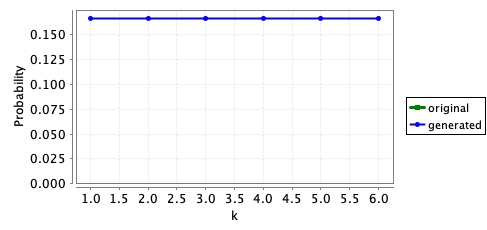
\includegraphics[scale=0.6]{example2-results.jpeg}	
\caption{Probability of reaching a state where $d=k$, for $k=1,\ldots,6.$}
\label{ex1-res}
\end{figure}
\begin{comment}
\subsection{Simple Peer-To-Peer Protocol}
This case study describes a simple peer-to-peer protocol based on BitTorrent\footnote{\url{https://www.prismmodelchecker.org/casestudies/peer2peer.php}}. The model comprises a set of clients trying to download a file that has been partitioned into $K$ blocks. Initially, there is one client that has already obtained all of the blocks and $N$ additional clients with no blocks. Each client can download a block from any of the others but they can only attempt four concurrent downloads for each block.\\
The code we analyze with $k=5$ and $N=4$ is reported in Listing \ref{ex2-code}.
\begin{lstlisting}[style=chor-color,caption={Choreographic language for the Peer-To-Peer Protocol.},captionpos=b,label={ex2-code}]
preamble
"ctmc"
"const double mu=2;"
"formula rate1=mu*(1+min(3,b11+b21+b31+b41));"
"formula rate2=mu*(1+min(3,b12+b22+b32+b42));"
"formula rate3=mu*(1+min(3,b13+b23+b33+b43));"
"formula rate4=mu*(1+min(3,b14+b24+b34+b44));"
"formula rate5=mu*(1+min(3,b15+b25+b35+b45));"
endpreamble

n = 4;
n = 4;

Client[i] $\rightarrow$ i in [1...n]
Client[i] : "b[i]1 : [0..1];", "b[i]2 : [0..1];", "b[i]3 : [0..1];", "b[i]4 : [0..1];", "b[i]5 : [0..1];" ;

{
PeerToPeer := Client[i] $\rightarrow$ Client[i]: 
			(+["rate1*1"]  "(b[i]1'=1)"$\&\&$" " . PeerToPeer
			 +["rate2*1"]  "(b[i]2'=1)"$\&\&$" " . PeerToPeer
			 +["rate3*1"]  "(b[i]3'=1)"$\&\&$" " . PeerToPeer
			 +["rate4*1"]  "(b[i]4'=1)"$\&\&$" " . PeerToPeer
			 +["rate5*1"]  "(b[i]5'=1)"$\&\&$" " . PeerToPeer)
}
	
\end{lstlisting}

Part of the generated PRISM code is shown in Listing \ref{ex2-gen} and it is faithful with what reported in the PRISM documentation. 
\begin{lstlisting}[style=prism-color,caption={Generated PRISM program for the Peer-To-Peer Protocol.},captionpos=b,label={ex2-gen}]
ctmc
const double mu=2;
formula rate1=mu*(1+min(3,b11+b21+b31+b41));
formula rate2=mu*(1+min(3,b12+b22+b32+b42));
formula rate3=mu*(1+min(3,b13+b23+b33+b43));
formula rate4=mu*(1+min(3,b14+b24+b34+b44));
formula rate5=mu*(1+min(3,b15+b25+b35+b45));

module Client1
	Client1 : [0..1] init 0;
	b11 : [0..1]; 
	b12 : [0..1]; 
	b13 : [0..1]; 
	b14 : [0..1]; 
	b15 : [0..1]; 

	[] (Client1=0)  $\rightarrow$ rate1 : (b11'=1)$\&$(Client1'=0); 
	[] (Client1=0)  $\rightarrow$ rate2 : (b12'=1)$\&$(Client1'=0); 
	[] (Client1=0)  $\rightarrow$ rate3 : (b13'=1)$\&$(Client1'=0); 
	[] (Client1=0)  $\rightarrow$ rate4 : (b14'=1)$\&$(Client1'=0); 
	[] (Client1=0)  $\rightarrow$ rate5 : (b15'=1)$\&$(Client1'=0); 
	
endmodule
	
\end{lstlisting}


In Figure \ref{ex2-res}, we compare the values obtained for the probability that all clients have received all blocks by time $0\leq T\leq 1.5$ both for our generated model and the model reported in the documentation.
\begin{figure}[h]
\centering
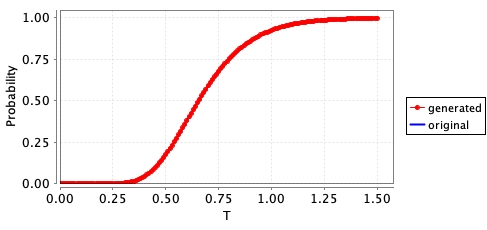
\includegraphics[scale=0.6]{example3-results.jpeg}	
\caption{Probability that clients received all the block before $T$, with $0\leq T \leq 1.5$.}
\label{ex2-res}
\end{figure}
\end{comment}
\newpage
\begin{comment}
\subsection{Random Graphs Protocol}
\begin{wrapfigure}[8]{l}{4cm}
	
\includegraphics[scale=0.7]{network.pdf}	
\end{wrapfigure} 
The second case study we report is the random graphs protocol presented in the PRISM documentation\footnote{\url{https://www.prismmodelchecker.org/casestudies/graph_connected.php}}.
It investigates the likelihood that a pair of nodes are connected in a
 random graph. More precisely, we take into account the the set of random graphs $G(n,p)$,
  i.e. the set of random graphs with $n$ nodes where the probability of there being an edge 
  between any two nodes equals $p$. 

  The model is divided in two parts: at the beginning the random graph is built.
Then the algorithm finds nodes that have a path to node 2 by searching for nodes for which one can reach (in one step) a node for which the existence of a path to node 2 has already been found.

The choreographic model is shown in Listing \ref{ex4-code}, while
in Listing \ref{ex4-gen}, we report only part of the generated PRISM module (the modules $M_2$, $M_3$ and $P_2$, $P_3$ are equivalent to, respectively, $M_1$ and $P_2$ and can be found in the repository\footnote{\url{https://github.com/adeleveschetti/choreography-to-PRISM}}).

\begin{lstlisting}[style=chor-color,breaklines=true, postbreak=\mbox{\textcolor{red}{$\hookrightarrow$}\space},caption={Choreographic language for the Random Graphs
	Protocol.},captionpos=b,label={ex4-code}]
preamble
"mdp"
"const double p;"
endpreamble

n = 3;

PC -> PC : " ";
M[i] -> i in [1...n]  M[i] : "varM[i] : bool;";
P[i] -> i in [1...n] P[i] : "varP[i] : bool;";

{
GraphConnected0 := 
	PC -> M[i] : (+["1*p"] " "&&"(varM[i]'=true)". END
		        +["1*(1-p)"] " "&&"(varM[i]'=false)". END)
	PC -> P[i] : (+["1*p"] " "&&"(varP[i]'=true)" . END
		        +["1*(1-p)"] " "&&"(varP[i]'=false)".
			if "(PC=6)&!varP[i]&((varP[i] & varM[i]) | (varM[i+1] & varP[i+2])) "@P[i] then {
				["1"]"(varP[i]'=true)"@P[i] . GraphConnected0
			}) 								  
}
\end{lstlisting}
\begin{lstlisting}[style=prism-color,caption={Generated PRISM program for the Random Graphs
	Protocol.},captionpos=b,label={ex4-gen}]
mdp
const double p;
	
module PC
   PC : [0..7] init 0;
	
   [DPPGR] (PC=0)  $\rightarrow$ 1 :  (PC'=1); 
   [YCJJG] (PC=1)  $\rightarrow$ 1 :  (PC'=2); 
   [TWGVA] (PC=2)  $\rightarrow$ 1 :  (PC'=3); 
   [NODPZ] (PC=3)  $\rightarrow$ 1 :  (PC'=4); 
   [FDALJ] (PC=4)  $\rightarrow$ 1 :  (PC'=5); 
   [DCKXC] (PC=5)  $\rightarrow$ 1 :  (PC'=6); 
endmodule

module M1
   M1 : [0..1] init 0;
   varM1 : bool; 

   [DPPGR] (M1=0)  $\rightarrow$ p :(varM1'=true)$\&$(M1'=0) + (1-p) :(varM1'=false)$\&$(M1'=0); 
endmodule	

$\ldots$

module P1
   P1 : [0..3] init 0;
   varP1 : bool; 

   [NODPZ] (P1=0)  $\rightarrow$ p:(varP1'=true)$\&$(P1'=0) + (1-p):(varP1'=false)$\&$(P1'=0); 
   [] (P1=0)$\&$(PC=6)$\&$!varP1&((varP1 $\&$ varM1) | (varM2$\&$ varP3))  
   				$\rightarrow$ 1 : (varP1'=true)$\&$(P1'=0); 
endmodule
$\ldots$
\end{lstlisting}

The model is very similar to the one presented in the PRISM repository, the main difference is that we use state variables also for the modules \texttt{P$_i$} and \texttt{M$_i$}, 
where in the original model they were not requires.
However, this does not affect the behaviour of the model, as the reader can notice from the results of the probability that nodes 1 and 2 are connected showed in Figure \ref{ex4-res}.
\begin{figure}[h]
\centering
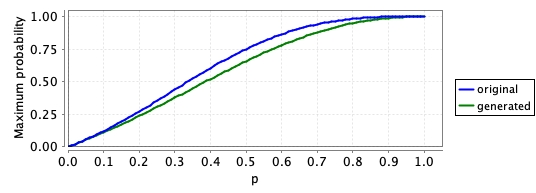
\includegraphics[scale=0.6]{example5-results.jpeg}	
\caption{Probability that the nodes 1 and 2 are connected.}
\label{ex4-res}
\end{figure}
\newpage
\end{comment}
\subsection{Proof of Work Bitcoin Protocol}
\begin{wrapfigure}[7]{r}{4cm}
	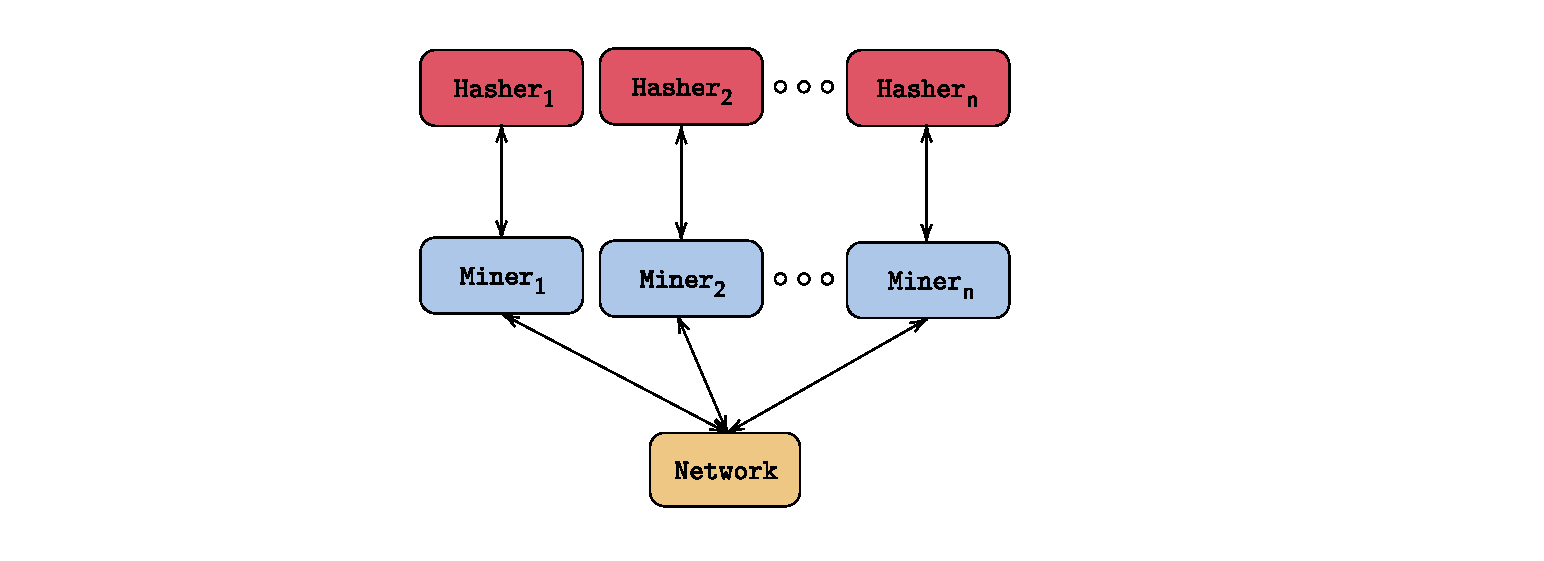
\includegraphics[scale=0.45]{bitcoin.pdf}	
\end{wrapfigure} 
In \cite{DBLP:journals/concurrency/BistarelliNGLMV23}, the authors decided to extend the PRISM model checker with
dynamic data types in order to model the Proof of Work protocol implemented in the Bitcoin blockchain \cite{bitcoin}.

The Bitcoin system is the result of the parallel composition of $n$ Miner processes, $n$  \emph{Hasher} processes and a process called \emph{Network}.
In particular: 
\begin{itemize}
	\item The \emph{Miner} processes model the blockchain mainers that create new blocks and add them to their local ledger;
	\item the \emph{Hasher} processes model the attempts of the miners to solve the cryptopuzzle;
	\item the \emph{Network} process model the broadcast communication among miners. 
\end{itemize}
Since we are not interested in the properties obtained by analyzing the protocol, we decided to consider $n=4$ miner and hasher processes; the model can be found in Listing \ref{ex3-code}.

\begin{lstlisting}[style=chor-color,breaklines=true, postbreak=\mbox{\textcolor{red}{$\hookrightarrow$}\space},caption={Choreographic language for the Proof of Work Bitcoin Protocol.},captionpos=b,label={ex3-code}]
preamble
$\ldots$
endpreamble

n = 4;

$\ldots$
	
{
PoW := Hasher[i]  ->  Miner[i] :
(+["mR*hR[i]"]  " "&&"(b[i]'=createB(b[i],B[i],c[i]))&(c[i]'=c[i]+1)" . 
	Miner[i]  ->  Network : 
		(["rB*1"] "(B[i]'=addBlock(B[i],b[i]))" && 
		foreach(k != i) "(set[k]'=addBlockSet(set[k],b[i]))" @Network .PoW)
 +["lR*hR[i]"] " " && " " .
 	if "!isEmpty(set[i])"@Miner[i] then { 
  		["r"] "(b[i]'=extractBlock(set[i]))"@Miner[i] . 
			Miner[i]  ->  Network : 
			(["1*1"] "(setMiner[i]' = addBlockSet(setMiner[i] , b[i]))"&&"(set[i]' = removeBlock(set[i],b[i]))" . PoW) 
 	}
 	else{
 		if "canBeInserted(B[i],b[i])"@Miner[i] then { 
 			["1"] "(B[i]'=addBlock(B[i],b[i]))&&(setMiner[i]'=removeBlock(setMiner[i],b[i]))"@Miner[i] . Pow 
 		}
 		else{
 			PoW
		}
	}
)
} 	
\end{lstlisting}

Part of the generated PRISM code is shown in Listing \ref{ex3-gen}, 
the modules $Miner_2$, $Miner_3$, $Miner_4$ and $Hasher_2$, $Hasher_3$, $Hasher_4$ are equivalent to $Miner_1$ and $Hasher_1$, respectively.
Our generated PRISM model is more verbose than the one presented in \cite{DBLP:journals/concurrency/BistarelliNGLMV23},
this is due to the fact that for the \texttt{if-then-else} expression, we always generate the \texttt{else} branch.
and this leads to having more instructions
\begin{lstlisting}[style=prism-color,caption={Generated PRISM program for the Peer-To-Peer Protocol.},captionpos=b,label={ex3-gen}]
$\ldots$

module Miner1
   Miner1 : [0..7] init 0;
   b1 : block {m1,0;genesis,0} ; 
   B1 : blockchain [{genesis,0;genesis,0}]; 
   c1 : [0..N] init 0; 
   setMiner1 : list []; 

   [PZKYT] (Miner1=0)   $\rightarrow$  hR1 : (b1'=createB(b1,B1,c1))$\&$(c1'=c1+1)$\&$(Miner1'=1); 
   [EUBVP] (Miner1=0)   $\rightarrow$  hR1 :  (Miner1'=2); 
   [HXYKO] (Miner1=1)   $\rightarrow$  1 : (B1'=addBlock(B1,b1))$\&$(Miner1'=0); 
   [] (Miner1=2)$\&$!isEmpty(set1)  $\rightarrow$  r : (b1'=extractBlock(set1))$\&$(Miner1'=4); 
   [SRKSV] (Miner1=4)   $\rightarrow$  1 : (setMiner1' = addBlockSet(setMiner1 , b1))$\&$(Miner1'=0); 
   [] (Miner1=2)$\&$!(!isEmpty(set1))  $\rightarrow$  1 : (Miner1'=5); 
   [] (Miner1=5)$\&$canBeInserted(B1,b1)  $\rightarrow$  1 : (B1'=addBlock(B1,b1))$\&$(setMiner1'=removeBlock(setMiner1,b1))$\&$(Miner1'=0); 
   [] (Miner1=5)$\&$!(canBeInserted(B1,b1))  $\rightarrow$  1 : (Miner1'=0);

endmodule
$\ldots$
module Network
Network : [0..1] init 0;
   set1 : list []; 
   $\ldots$

   [HXYKO] (Network=0)  $\rightarrow$  1 : (set2'=addBlockSet(set2,b2))$\&$(set3'=addBlockSet(set3,b3))$\&$(set4'=addBlockSet(set4,b4))$\&$(Network'=0); 
   [SRKSV] (Network=0)  $\rightarrow$  1 : (set1' = removeBlock(set1,b1))$\&$(Network'=0); 
   $\ldots$

endmodule

module Hasher1
Hasher1 : [0..1] init 0;

[PZKYT] (Hasher1=0)  $\rightarrow$  mR :  (Hasher1'=0); 
[EUBVP] (Hasher1=0)  $\rightarrow$  lR :  (Hasher1'=0); 

endmodule
\end{lstlisting}

However, for this particular test case, the results of the experiments are not affected, 
as shown Figure \ref{ex3-res} where the results are compared.
In this example, since we are comparing the results of two simulations, the two probabilities are
slightly different, but it has nothing to do with the model itself.
\begin{figure}[h]
\centering
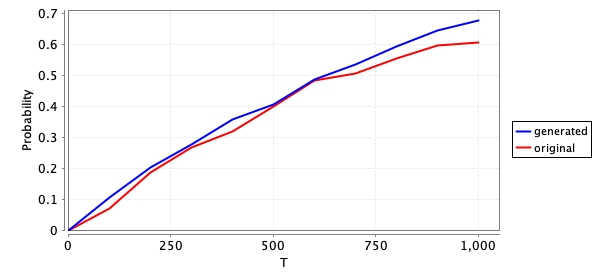
\includegraphics[scale=0.5]{example4-results.jpeg}	
\caption{Probability at least one miner has created a block.}
\label{ex3-res}
\end{figure}


\subsection{Hybrid Casper Protocol}
\begin{wrapfigure}[9]{l}{4.5cm}
	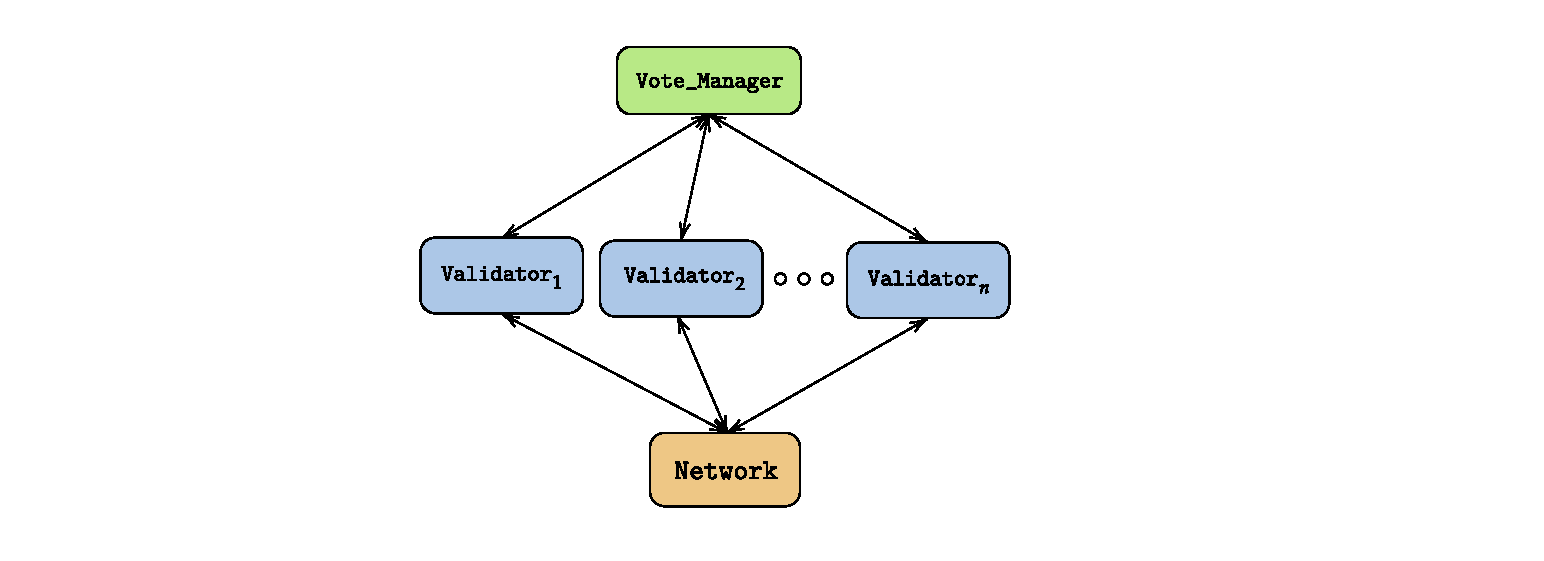
\includegraphics[scale=0.45]{ethereum.pdf}	
\end{wrapfigure} 
The last case we study we present is the Hybrid Casper Protocol modelled in PRISM in \cite{DBLP:journals/distribledger/GallettaLMV23}. 
The Hybrid Capser protocol is
an hybrid blockchain consenus protocol that includes features of the Proof of Work and the Proof of Stake protocols.
It was implemented in the Ethereum blockchain \cite{ethereum} as a testing phase before switching to Proof of Stake protocol.

The approach is very similat to the one used for the Proof of Work Bitcoin protocol,
so they model Hybrid Casper in PRISM as the parallel composition of $n$ \texttt{Validator} modules and the modules \texttt{Vote\_Manager} and \texttt{Network}.
The module \texttt{Validator} is very similar to the module \texttt{Miner} of the previous protocol and
the only module that requires an explaination is the \texttt{Vote\_Manager} that stores the tables containing the votes for each checkpoint and calculates the rewards/penalties.

The modeling language is reported in Listing \ref{ex5-code} while (part of) the generated PRISM code can be found in Listing \ref{ex5-gen}.
\begin{lstlisting}[style=chor-color,tabsize=2,breaklines=true, postbreak=\mbox{\textcolor{red}{$\hookrightarrow$}\space},	caption={Choreographic language for the Hybrid Casper Protocol.},captionpos=b,label={ex5-code}]
preamble
$\ldots$
endpreamble
n = 5;
$\ldots$
{
PoS := Validator[i] -> Validator[i] :
   (+["mR*1"]  "(b[i]'=createB(b[i],L[i],c[i]))&(c[i]'=c[i]+1)"&&" " .
	if "!(mod(getHeight(b[i]),EpochSize)=0)"@Validator[i] then{
	   Validator[i] -> Network : (["1*1"] "(L[i]'=addBlock(L[i],b[i]))" && foreach(k!=i) "(set[k]'=addBlockSet(set[k],b[i]))"@Network .PoS)
	}
	else{
	   Validator[i] -> Network : (["1*1"] "(L[i]'=addBlock(L[i],b[i]))" && foreach(k!=i) "(set[k]'=addBlockSet(set[k],b[i]))"@Network . Validator[i] -> Vote_Manager :(["1*1"] " "&&"(Votes'=addVote(Votes,b[i],stake[i]))".PoS))
	}
   +["lR*1"] " "&&" " . if "!isEmpty(set[i])"@Validator[i] then {
	   ["1"] "(b[i]'=extractBlock(set[i]))"@Validator[i] . 
		   if "!canBeInserted(L[i],b[i])"@Validator[i] then {
		       PoS
		   }
		   else{
			if "!(mod(getHeight(b[i]),EpochSize)=0)"@Validator[i] then {
			  Validator[i] -> Network : (["1*1"] "(setMiner[i]' = addBlockSet(setMiner[i] , b[i]))"&&"(set[i]' = removeBlock(set[i],b[i]))" . PoS)
			}
			else{
			  Validator[i] -> Network : (["1*1"] "(setMiner[i]' = addBlockSet(setMiner[i] , b[i]))"&&"(set[i]' = removeBlock(set[i],b[i]))" . Validator[i] -> Vote_Manager : (["1*1"] " "&&"(Votes'=addVote(Votes,b[i],stake[i]))".PoS ))
			}
		}
	}
	else{PoS}
   +["rC*1"] "(lastCheck[i]'=extractCheckpoint(listCheckpoints[i],lastCheck[i]))&(heightLast[i]'=getHeight(extractCheckpoint(listCheckpoints[i],lastCheck[i])))&(votes[i]'=calcVotes(Votes,extractCheckpoint(listCheckpoints[i],lastCheck[i])))"&&" " . 
	   if "(heightLast[i]=heightCheckpoint[i]+EpochSize)&(votes[i]>=2/3*tot_stake)"@Validator[i] then{
		   if "(heightLast[i]=heightCheckpoint[i]+EpochSize)"@Validator[i] then{
			   ["1"] "(lastJ[i]'=b[i])&(L[i]'= updateHF(L[i],lastJ[i]))" @Validator[i].Validator[i]->Vote_Manager :(["1*1"]" "&&"(epoch'=height(lastF(L[i]))&(Stakes'=addVote(Votes,b[i],stake[i]))".PoS)
		   }
		   else{["1"] "(lastJ[i]'=b[i])"@Validator[i] . PoS} 
	   }
	   else{PoS}
)								 
}	
\end{lstlisting}

\begin{lstlisting}[style=prism-color,caption={Generated PRISM program for the Hybrid Casper	Protocol.},captionpos=b,label={ex5-gen}]
module Validator1
   $\ldots$
	
   [] (Validator1=0)  $\rightarrow$  mR : (b1'=createB(b1,L1,c1))$\&$(c1'=c1+1)&(Validator1'=1); 
   [] (Validator1=0)  $\rightarrow$  lR :  (Validator1'=2); 
   [] (Validator1=0)$\&$(!isEmpty(listCheckpoints1))  $\rightarrow$  
   	rC : (lastCheck1'=extractCheckpoint(listCheckpoints1,lastCheck1))$\&$(heightLast1'=getHeight(extractCheckpoint(listCheckpoints1,lastCheck1)))$\&$(votes1'=calcVotes(Votes,extractCheckpoint(listCheckpoints1,lastCheck1)))$\&$(Validator1'=3); 
   [NGRDF] (Validator1=1)$\&$!(mod(getHeight(b1),EpochSize)=0)  $\rightarrow$  1 : (L1'=addBlock(L1,b1))$\&$(Validator1'=0); 
   [] (Validator1=1)$\&$!(!(mod(getHeight(b1),EpochSize)=0)) $\rightarrow$  1 : (Validator1'=3); 
   [PCRLD] (Validator1=1)$\&$!(mod(getHeight(b1),EpochSize)=0)  $\rightarrow$  
   	1 : (L1'=addBlock(L1,b1))$\&$(Validator1'=4); 
   [VSJBE] (Validator1=5)  $\rightarrow$  1 :  (Validator1'=0); 
   [] (Validator1=2)$\&$!isEmpty(set1) $\rightarrow$  
   	1 : (b1'=extractBlock(set1))$\&$(Validator1'=4); 
   [] (Validator1=4)$\&$!canBeInserted(L1,b1) $\rightarrow$  (Validator1'=0);
   [] (Validator1=4)$\&$!(!canBeInserted(L1,b1)) $\rightarrow$  1 : (Validator1'=6); 
   [MDDCF] (Validator1=6)$\&$!(mod(getHeight(b1),EpochSize)=0)  $\rightarrow$ 
   	1 : (setMiner1' = addBlockSet(setMiner1 , b1))$\&$(Validator1'=0); 
   [] (Validator1=6)$\&$!(!(mod(getHeight(b1),EpochSize)=0)) $\rightarrow$  1 : (Validator1'=8); 
   [IQVPA] (Validator1=6)$\&$!(mod(getHeight(b1),EpochSize)=0)  $\rightarrow$  
   	1 : (setMiner1' = addBlockSet(setMiner1 , b1))$\&$(Validator1'=9); 
   [IFNVZ] (Validator1=10)  $\rightarrow$  1 :  (Validator1'=0); 
   [] (Validator1=2)$\&$!(!isEmpty(set1)) $\rightarrow$  1 : (Validator1'=0);
   [] (Validator1=3)$\&$(heightLast1=heightCheckpoint1+EpochSize)$\&$(votes1>=2/3*tot_stake) $\rightarrow$  (Validator1'=4);
   [] (Validator1=4)$\&$(heightLast1=heightCheckpoint1+EpochSize) $\rightarrow$  
   	1 : (lastJ1'=b1)$\&$(L1'= updateHF(L1,lastJ1))$\&$(Validator1'=6); 
   [EQCYO] (Validator1=6)  $\rightarrow$  1 :  (Validator1'=0); 
   [] (Validator1=4)$\&$!((heightLast1=heightCheckpoint1+EpochSize)) $\rightarrow$  
   	1 : (lastJ1'=b1)$\&$(Validator1'=0); 
   [] (Validator1=3)$\&$!((heightLast1=heightCheckpoint1+EpochSize)$\&$(votes1>=2/3*tot_stake)) $\rightarrow$  1 : (Validator1'=0);
endmodule
$\ldots$
module Network
   Network : [0..1] init 0;
   set1 : list []; 
   set2 : list []; 
   set3 : list []; 
   set4 : list []; 
   set5 : list []; 

   [NGRDF] (Network=0)  $\rightarrow$  
   	1 : (set2'=addBlockSet(set2,b2))$\&$(set3'=addBlockSet(set3,b3))$\&$(set4'=addBlockSet(set4,b4))$\&$(set5'=addBlockSet(set5,b5))$\&$(Network'=0); 
   [PCRLD] (Network=0)  $\rightarrow$  
   	1 : (set2'=addBlockSet(set2,b2))$\&$(set3'=addBlockSet(set3,b3))$\&$(set4'=addBlockSet(set4,b4))$\&$(set5'=addBlockSet(set5,b5))$\&$(Network'=0); 
   [MDDCF] (Network=0)  $\rightarrow$  1 : (set1' = removeBlock(set1,b1))$\&$(Network'=0); 
   [IQVPA] (Network=0)  $\rightarrow$  1 : (set1' = removeBlock(set1,b1))$\&$(Network'=0); 
   $\ldots$
endmodule

module Vote_Manager
   Vote_Manager : [0..1] init 0;
   epoch : [0..10] init 0;
   Votes : hash[];  
   tot_stake : [0..120000] init 50; 
   stake1 : [0..N] init 10; 
   stake2 : [0..N] init 10; 
   stake3 : [0..N] init 10; 
   stake4 : [0..N] init 10; 
   stake5 : [0..N] init 10; 

   [VSJBE] (Vote_Manager=0)  $\rightarrow$  
   	1 : (Votes'=addVote(Votes,b1,stake1))$\&$(Vote_Manager'=0); 
   $\ldots$
endmodule

\end{lstlisting}

The code is very similar to the one presented in \cite{DBLP:journals/distribledger/GallettaLMV23},
the main difference is the fact that our generated model has more lines of code.
This is due to the fact that there are some commands that can be merged, but the compiler is not able to do it automatically.
This discrepancy between the two models can be observed also in the simulations, reported in Figure \ref{ex5-res}.
Although the results are similar, PRISM takes 39.016 seconds to run the simulations for the generated model, 
instead of 22.051 seconds needed for the original model.

\begin{figure}[h]
\centering
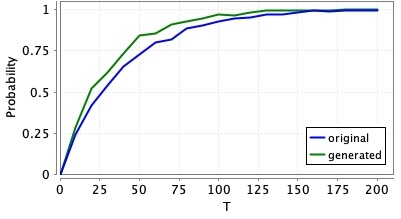
\includegraphics[scale=0.6]{example6-results.jpeg}	
\caption{Probability that a block has been created.}
\label{ex5-res}
\end{figure}



\subsection{Problems}
While testing our choreographic language, we noticed that some of the case studies presented in the 
PRISM documentation \cite{PRISMdoc} cannot be modeled by using our language.
The reasons are various, in this section we try to outline the problems.

\begin{itemize}
\item \textbf{Asynchronous Leader Election}\footnote{\url{https://www.prismmodelchecker.org/casestudies/asynchronous_leader.php}}:
 processes synchronize with the same label but the conditions are different.
 We include in our language the \texttt{it-then-else} statement but we do not allow 
 the \texttt{if-then} (without the \texttt{else}). This is done because in this way, we do not 
 incur in deadlock states.
\item  \textbf{Probabilistic Broadcast Protocols}\footnote{\url{https://www.prismmodelchecker.org/casestudies/prob_broadcast.php}}:
 also in this case, the problem are the labels of the synchronizations.
 In fact, all the processes synchornize with the same label on every actions.
 This is not possible in our language, since a label is unique for every synchronization between two (or more) processes.
\item \textbf{Cyclic Server Polling System}\footnote{\url{https://www.prismmodelchecker.org/casestudies/polling.php}}:
 in this model, the processes \texttt{station$_i$} do two different things in the same state.
 More precicely, at the state 0 (\texttt{s$_i$=0}), the processes may synchornize with the process
 \texttt{server} or may change their state without any synchronization.
 In out language, this cannot be formalized since the synchronization is a branch action,
 so there should be another option with a synchronization.


\end{itemize}